\chapter{Desarrollo del código}
\label{chap:desarrollo-codigo}
En la figura \ref{fig:orgefeff38}, se muestra el proceso de cálculo que sigue el paquete a la hora de obtener la estimación de la producción del sistema fotovoltaico.
\begin{figure}[]
\centering
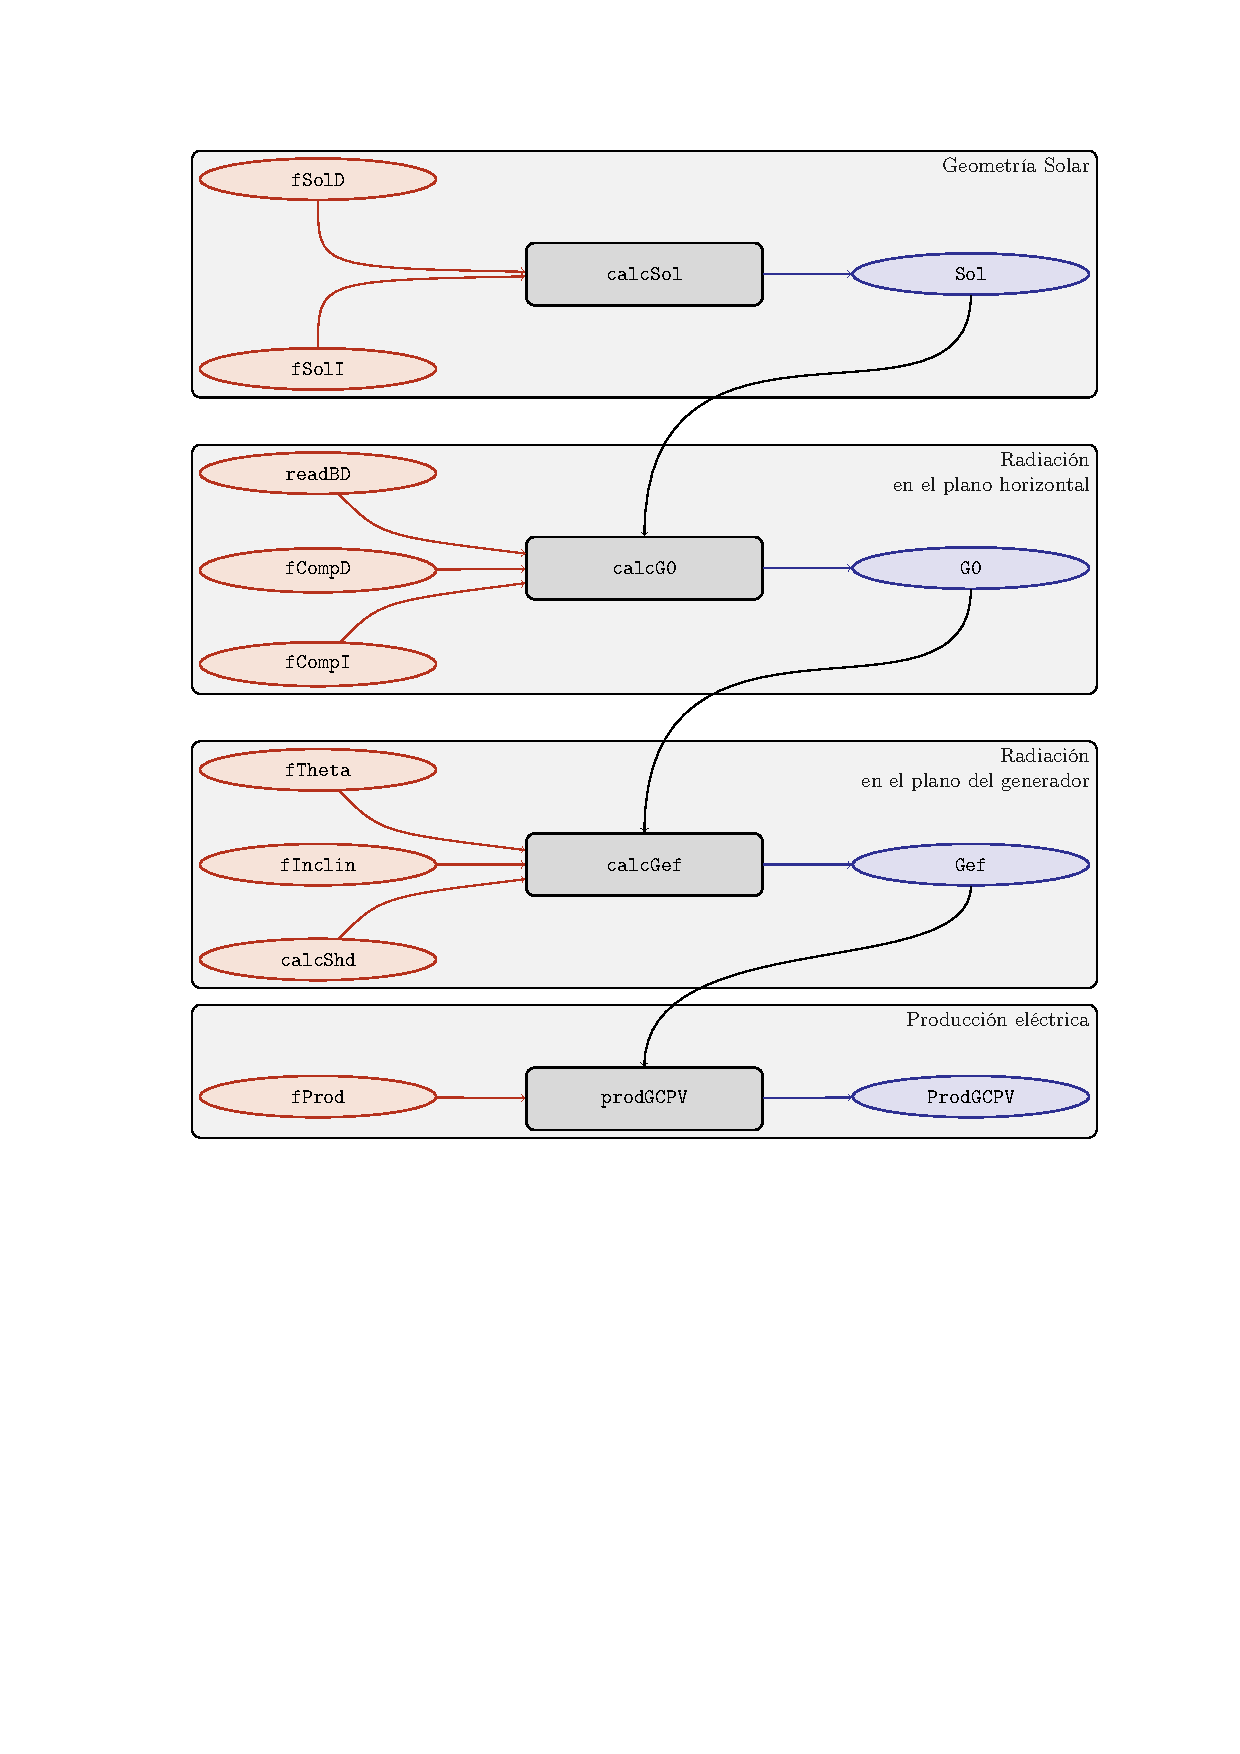
\includegraphics[keepaspectratio,width=0.8\textwidth,height=0.5\textheight]{figuras/procedure.pdf}
\caption{\label{fig:orgefeff38}Proceso de cálculo de las funciones de \texttt{solaR2}}
\end{figure}
A la hora de estimar la producción, el programa sigue los siguientes procesos:
\section{Geometría solar.}
\label{sec:org38b25ae}
\label{sec:geometria-solar}
Para calcular la geometría que definen las posiciones de la Tierra y el Sol, \texttt{solaR2} se vale de una función constructora, \texttt{calcSol} [\ref{subsec:calcsol}], la cual mediante las funciones \texttt{fSolD} [\ref{subsec:fsold}] y \texttt{fSolI} [\ref{subsec:fsoli}] cálcula todos los ángulos y componentes que caracterizan la geometría solar.
\begin{figure}[]
\centering
\includegraphics[keepaspectratio,width=\textwidth,height=0.5\textheight]{figuras/calcSol.pdf}
\caption{Cálculo de la geometría solar mediante la función \texttt{calcSol}, la cual unifica las funciones \texttt{fSolD} y \texttt{fSolI} resultando en un objeto clase \texttt{Sol} el cual contiene toda la información geométrica necesaria para realizar las siguientes estimaciones. \label{fig:calcSol}}
\end{figure}
Como se puede ver en la figura \ref{fig:calcSol}, \texttt{calcSol} funciona gracias a dos funciones:
\begin{itemize}
\item \texttt{fSolD}: la cual, a partir de la latitud (\(\phi\)), computa la geometría a nivel diario, es decir, los ángulos y componentes que se pueden calcular en cada día independiente.

estas son:
\begin{itemize}
\item Declinación (\(\delta\)): calculada a partir de la función \texttt{declination}\footnote{Todas las funciones mencionadas en este punto, se encuentran en el apartado \ref{subsec:utils-angles}.}.
\item Excentricidad (\(\epsilon_o\)): obtenida mediante la función \texttt{eccentricity}.
\item Ecuación del tiempo (\(EoT\)): obtenida mediante la función \texttt{eot}.
\item Ángulo del amanecer (\(\omega_s\)): calculada a partir de la función \texttt{sunrise}.
\item Irradiancia diaria extra-atmosférica (\(B_{0d}(0)\)): obtenida a paritr de la función \texttt{bo0d}.
\end{itemize}
\end{itemize}
\begin{lstlisting}[numbers=left,language=r,label= ,caption= ,captionpos=b]
lat <- 40
BTd <- fBTd(mode = 'prom')
solD <- fSolD(lat = lat, BTd = BTd)
show(solD)
\end{lstlisting}

\begin{verbatim}
Key: <Dates>
         Dates   lat        decl        eo           EoT        ws      Bo0d
        <IDat> <num>       <num>     <num>         <num>     <num>     <num>
 1: 2024-01-17    40 -0.36271754 1.0340422 -0.0455346238 -1.246707  4260.913
 2: 2024-02-14    40 -0.22850166 1.0259717 -0.0614793356 -1.374392  5696.512
 3: 2024-03-15    40 -0.03191616 1.0107943 -0.0368674274 -1.544003  7744.914
 4: 2024-04-15    40  0.17531794 0.9926547  0.0017482721 -1.719984  9731.571
 5: 2024-05-15    40  0.33246485 0.9775162  0.0143055938 -1.864736 11068.270
 6: 2024-06-10    40  0.40257826 0.9691480 -0.0007378952 -1.936192 11597.374
 7: 2024-07-18    40  0.36439367 0.9675489 -0.0263454380 -1.896584 11241.588
 8: 2024-08-18    40  0.22407398 0.9758022 -0.0111761118 -1.763213 10037.033
 9: 2024-09-18    40  0.02730595 0.9907919  0.0342189964 -1.593716  8210.584
10: 2024-10-19    40 -0.17900474 1.0088406  0.0689613044 -1.418379  6139.354
11: 2024-11-18    40 -0.33862399 1.0245012  0.0575423573 -1.270794  4482.035
12: 2024-12-13    40 -0.40478283 1.0328516  0.0158622941 -1.203058  3802.318
\end{verbatim}

Además, \texttt{fSolD} permite seleccionar el método de cáculo entre los propuestos por 4 autores diferentes (\texttt{cooper} \cite{Cooper1969}, \texttt{spencer} \cite{Spencer1971}, \texttt{strous} \cite{Strous2011}, \texttt{michalsky} \cite{Michalsky1988})(el valor por defecto es \texttt{michalsky}):
\begin{lstlisting}[numbers=left,language=r,label= ,caption= ,captionpos=b]
solD_cooper <- fSolD(lat = lat, BTd = BTd, method = 'cooper')
show(solD_cooper)
\end{lstlisting}

\begin{verbatim}
Key: <Dates>
         Dates   lat        decl        eo           EoT        ws      Bo0d
        <IDat> <num>       <num>     <num>         <num>     <num>     <num>
 1: 2024-01-17    40 -0.36506987 1.0315970 -0.0455346238 -1.244322  4225.330
 2: 2024-02-14    40 -0.23770977 1.0235842 -0.0614793356 -1.366063  5581.840
 3: 2024-03-15    40 -0.04219743 1.0091112 -0.0368674274 -1.535360  7621.789
 4: 2024-04-15    40  0.17074888 0.9917107  0.0017482721 -1.715990  9677.015
 5: 2024-05-15    40  0.33214647 0.9770196  0.0143055938 -1.864424 11059.743
 6: 2024-06-10    40  0.40292516 0.9690335 -0.0007378952 -1.936560 11599.039
 7: 2024-07-18    40  0.36346384 0.9684861 -0.0263454380 -1.895642 11244.195
 8: 2024-08-18    40  0.21721704 0.9778484 -0.0111761118 -1.757060  9992.309
 9: 2024-09-18    40  0.01056696 0.9933706  0.0342189964 -1.579664  8057.402
10: 2024-10-19    40 -0.19902155 1.0107363  0.0689613044 -1.400739  5932.854
11: 2024-11-18    40 -0.34965673 1.0247443  0.0575423573 -1.259840  4363.600
12: 2024-12-13    40 -0.40651987 1.0315970  0.0158622941 -1.201207  3779.136
\end{verbatim}

\begin{lstlisting}[numbers=left,language=r,label= ,caption= ,captionpos=b]
solD_spencer <- fSolD(lat = lat, BTd = BTd, method = 'spencer')
show(solD_spencer)
\end{lstlisting}

\begin{verbatim}
Key: <Dates>
         Dates   lat        decl        eo           EoT        ws      Bo0d
        <IDat> <num>       <num>     <num>         <num>     <num>     <num>
 1: 2024-01-17    40 -0.36483670 1.0340422 -0.0455346238 -1.244559  4237.879
 2: 2024-02-14    40 -0.23199205 1.0259717 -0.0614793356 -1.371241  5657.973
 3: 2024-03-15    40 -0.03563921 1.0107943 -0.0368674274 -1.540874  7704.956
 4: 2024-04-15    40  0.17171286 0.9926547  0.0017482721 -1.716832  9695.800
 5: 2024-05-15    40  0.33007088 0.9775162  0.0143055938 -1.862390 11046.417
 6: 2024-06-10    40  0.40208757 0.9691480 -0.0007378952 -1.935671 11593.079
 7: 2024-07-18    40  0.36657157 0.9675489 -0.0263454380 -1.898797 11260.952
 8: 2024-08-18    40  0.22748717 0.9758022 -0.0111761118 -1.766286 10069.634
 9: 2024-09-18    40  0.03143967 0.9907919  0.0342189964 -1.597189  8253.467
10: 2024-10-19    40 -0.17549393 1.0088406  0.0689613044 -1.421454  6177.523
11: 2024-11-18    40 -0.33679169 1.0245012  0.0575423573 -1.272602  4501.910
12: 2024-12-13    40 -0.40419949 1.0328516  0.0158622941 -1.203679  3808.563
\end{verbatim}

\begin{lstlisting}[numbers=left,language=r,label= ,caption= ,captionpos=b]
solD_strous <- fSolD(lat = lat, BTd = BTd, method = 'cooper')
show(solD_strous)
\end{lstlisting}

\begin{verbatim}
Key: <Dates>
         Dates   lat        decl        eo           EoT        ws      Bo0d
        <IDat> <num>       <num>     <num>         <num>     <num>     <num>
 1: 2024-01-17    40 -0.36506987 1.0315970 -0.0455346238 -1.244322  4225.330
 2: 2024-02-14    40 -0.23770977 1.0235842 -0.0614793356 -1.366063  5581.840
 3: 2024-03-15    40 -0.04219743 1.0091112 -0.0368674274 -1.535360  7621.789
 4: 2024-04-15    40  0.17074888 0.9917107  0.0017482721 -1.715990  9677.015
 5: 2024-05-15    40  0.33214647 0.9770196  0.0143055938 -1.864424 11059.743
 6: 2024-06-10    40  0.40292516 0.9690335 -0.0007378952 -1.936560 11599.039
 7: 2024-07-18    40  0.36346384 0.9684861 -0.0263454380 -1.895642 11244.195
 8: 2024-08-18    40  0.21721704 0.9778484 -0.0111761118 -1.757060  9992.309
 9: 2024-09-18    40  0.01056696 0.9933706  0.0342189964 -1.579664  8057.402
10: 2024-10-19    40 -0.19902155 1.0107363  0.0689613044 -1.400739  5932.854
11: 2024-11-18    40 -0.34965673 1.0247443  0.0575423573 -1.259840  4363.600
12: 2024-12-13    40 -0.40651987 1.0315970  0.0158622941 -1.201207  3779.136
\end{verbatim}

\begin{itemize}
\item \texttt{fSolI}: toma los resultados obtenidos en \texttt{fSolD} y calcula la geometría a nivel intradiario, es decir, aquella que se puede calcular en unidades de tiempo menores a los días.

estas son:
\begin{itemize}
\item La hora solar o tiempo solar verdadero (\(\omega\)): calculada a partir de la función \texttt{sunHour}.
\item Los momentos del día en los que es de noche (\(night\)): calculada a partir del resultado anterior y de el ángulo del amanecer (cálculada en \texttt{fSolD})\footnote{Cuando la hora solar verdadera excede los ángulos en los que amanece y anochece (\(|\omega|>=|\omega_s|\)), el Sol queda por debajo de la línea del horizonte, por lo que es de noche.}.
\item El coseno del ángulo cenital solar (\(cos(\theta_{zs})\)): obtenida a partir de la función \texttt{zenith}.
\item La altura solar (\(\gamma_s\)): obtenida a partir del resultado anterior\footnote{\(\gamma_s=asin(cos(\theta_s))\).}.
\item El ángulo zenital solar (\(\theta_{zs}\)): calculada mediante la función \texttt{azimuth}.
\item La irradiancia extra-atmosférica (\(B_0(0)\)): calculada mediante el coseno del ángulo cenital, la constante solar (\(B_0\)) y la excentridad (cálculada en \texttt{fSolD}) [ecuación \ref{eq:irrad_horiz}].
\end{itemize}
\end{itemize}
\begin{lstlisting}[numbers=left,language=r,label= ,caption= ,captionpos=b]
solI <- fSolI(solD = solD[1], sample = 'hour') #Computo solo un día a fin de poder de mejorar la visualización
show(solI)
\end{lstlisting}

\begin{verbatim}
Index: <night>
                  Dates   lat           w  night     cosThzS         AlS         AzS      Bo0
                 <POSc> <num>       <num> <lgcl>       <num>       <num>       <num>    <num>
 1: 2024-01-17 00:00:00    40  3.09905026   TRUE -0.94362605 -1.23341900  3.02117859   0.0000
 2: 2024-01-17 01:00:00    40 -2.92239722   TRUE -0.92713728 -1.18669958 -2.56815069   0.0000
 3: 2024-01-17 02:00:00    40 -2.66065932   TRUE -0.86303058 -1.04123862 -2.11373529   0.0000
 4: 2024-01-17 03:00:00    40 -2.39892132   TRUE -0.75567263 -0.85668051 -1.83479587   0.0000
 5: 2024-01-17 04:00:00    40 -2.13718324   TRUE -0.61237625 -0.65906286 -1.63492717   0.0000
 6: 2024-01-17 05:00:00    40 -1.87544507   TRUE -0.44290226 -0.45883317 -1.46851718   0.0000
 7: 2024-01-17 06:00:00    40 -1.61370681   TRUE -0.25879466 -0.26177415 -1.31325645   0.0000
 8: 2024-01-17 07:00:00    40 -1.35196846   TRUE -0.07259424 -0.07265815 -1.15564315   0.0000
 9: 2024-01-17 08:00:00    40 -1.09023003  FALSE  0.10301563  0.10319871 -0.98536387 145.6163
10: 2024-01-17 09:00:00    40 -0.82849151  FALSE  0.25607296  0.25895750 -0.79338297 361.9683
11: 2024-01-17 10:00:00    40 -0.56675290  FALSE  0.37615192  0.38563969 -0.57251788 531.7042
12: 2024-01-17 11:00:00    40 -0.30501420  FALSE  0.45507309  0.47245429 -0.32078152 643.2621
13: 2024-01-17 12:00:00    40 -0.04327541  FALSE  0.48746054  0.50917897 -0.04634006 689.0429
14: 2024-01-17 13:00:00    40  0.21846346  FALSE  0.47110809  0.49054659  0.23178786 665.9281
15: 2024-01-17 14:00:00    40  0.48020243  FALSE  0.40712958  0.41930919  0.49254063 575.4922
16: 2024-01-17 15:00:00    40  0.74194148  FALSE  0.29988299  0.30457000  0.72379629 423.8953
17: 2024-01-17 16:00:00    40  1.00368062  FALSE  0.15667361  0.15732176  0.92469276 221.4637
18: 2024-01-17 17:00:00    40  1.26541985   TRUE -0.01274358 -0.01274392  1.10120336   0.0000
19: 2024-01-17 18:00:00    40  1.52715917   TRUE -0.19682837 -0.19812195  1.26194203   0.0000
20: 2024-01-17 19:00:00    40  1.78889857   TRUE -0.38304142 -0.39308659  1.41671214   0.0000
21: 2024-01-17 20:00:00    40  2.05063807   TRUE -0.55869839 -0.59281557  1.57757727   0.0000
22: 2024-01-17 21:00:00    40  2.31237766   TRUE -0.71183398 -0.79210598  1.76293575   0.0000
23: 2024-01-17 22:00:00    40  2.57411733   TRUE -0.83201697 -0.98273364  2.00815884   0.0000
24: 2024-01-17 23:00:00    40  2.83585709   TRUE -0.91106075 -1.14584973  2.39029855   0.0000
                  Dates   lat           w  night     cosThzS         AlS         AzS      Bo0
\end{verbatim}

Además, como los datos nocturnos aportan poco a los cálculos que atañen a este proyecto, \texttt{fSolI} presenta la posibilidad de eliminar estos datos con el argumento \texttt{keep.night}.
\begin{lstlisting}[numbers=left,language=r,label= ,caption= ,captionpos=b]
solI_nigth <- fSolI(solD = solD[1], sample = 'hour', keep.night = FALSE)
show(solI_nigth)
\end{lstlisting}

\begin{verbatim}
                 Dates   lat           w  night   cosThzS       AlS         AzS      Bo0
                <POSc> <num>       <num> <lgcl>     <num>     <num>       <num>    <num>
1: 2024-01-17 08:00:00    40 -1.09023003  FALSE 0.1030156 0.1031987 -0.98536387 145.6163
2: 2024-01-17 09:00:00    40 -0.82849151  FALSE 0.2560730 0.2589575 -0.79338297 361.9683
3: 2024-01-17 10:00:00    40 -0.56675290  FALSE 0.3761519 0.3856397 -0.57251788 531.7042
4: 2024-01-17 11:00:00    40 -0.30501420  FALSE 0.4550731 0.4724543 -0.32078152 643.2621
5: 2024-01-17 12:00:00    40 -0.04327541  FALSE 0.4874605 0.5091790 -0.04634006 689.0429
6: 2024-01-17 13:00:00    40  0.21846346  FALSE 0.4711081 0.4905466  0.23178786 665.9281
7: 2024-01-17 14:00:00    40  0.48020243  FALSE 0.4071296 0.4193092  0.49254063 575.4922
8: 2024-01-17 15:00:00    40  0.74194148  FALSE 0.2998830 0.3045700  0.72379629 423.8953
9: 2024-01-17 16:00:00    40  1.00368062  FALSE 0.1566736 0.1573218  0.92469276 221.4637
\end{verbatim}

Finalmente, estas dos funciones, como se muestra en la figura \ref{fig:calcSol}, convergen en la función \texttt{calcSol}, dando como resultado un objeto de clase \texttt{Sol}. Este objeto muestra un sumario de ambos elementos junto con la latitud de los cálculos.
\begin{lstlisting}[numbers=left,language=r,label= ,caption= ,captionpos=b]
sol <- calcSol(lat = lat, BTd = BTd, sample = 'hour')
show(sol)
\end{lstlisting}

\begin{verbatim}
Object of class Sol 

Latitude:  40 degrees

Daily values:
     Dates                 decl                 eo              EoT                   ws        
 Min.   :2024-01-17   Min.   :-0.404783   Min.   :0.9675   Min.   :-0.0614793   Min.   :-1.936  
 1st Qu.:2024-04-07   1st Qu.:-0.256032   1st Qu.:0.9771   1st Qu.:-0.0289759   1st Qu.:-1.789  
 Median :2024-06-29   Median :-0.002305   Median :1.0007   Median : 0.0005052   Median :-1.569  
 Mean   :2024-07-01   Mean   :-0.001618   Mean   :1.0009   Mean   : 0.0008748   Mean   :-1.569  
 3rd Qu.:2024-09-25   3rd Qu.: 0.251172   3rd Qu.:1.0249   3rd Qu.: 0.0204515   3rd Qu.:-1.348  
 Max.   :2024-12-13   Max.   : 0.402578   Max.   :1.0340   Max.   : 0.0689613   Max.   :-1.203  
      Bo0d      
 Min.   : 3802  
 1st Qu.: 5393  
 Median : 7978  
 Mean   : 7834  
 3rd Qu.:10295  
 Max.   :11597  

Intradaily values: 
     Dates                           w                night            cosThzS         
 Min.   :2024-01-17 00:00:00   Min.   :-3.1393050   Mode :logical   Min.   :-0.957052  
 1st Qu.:2024-04-07 11:45:00   1st Qu.:-1.5692285   FALSE:145       1st Qu.:-0.469842  
 Median :2024-06-29 11:30:00   Median : 0.0010871   TRUE :143       Median : 0.005586  
 Mean   :2024-07-01 15:30:00   Mean   : 0.0009975                   Mean   :-0.001012  
 3rd Qu.:2024-09-26 11:15:00   3rd Qu.: 1.5716412                   3rd Qu.: 0.472405  
 Max.   :2024-12-13 23:00:00   Max.   : 3.1413972                   Max.   : 0.956640  
      AlS                 AzS                 Bo0          
 Min.   :-1.276658   Min.   :-3.139232   Min.   :   0.000  
 1st Qu.:-0.489119   1st Qu.:-1.572101   1st Qu.:   0.000  
 Median : 0.005586   Median : 0.003240   Median :   7.746  
 Mean   :-0.001250   Mean   : 0.001007   Mean   : 326.418  
 3rd Qu.: 0.492019   3rd Qu.: 1.571070   3rd Qu.: 663.617  
 Max.   : 1.275239   Max.   : 3.141341   Max.   :1267.381
\end{verbatim}

\section{Datos meteorológicos}
\label{sec:orgf155322}
\label{sec:datos-meteorologicos}
Para el procesamiento de datos meteorologicos, \texttt{solaR2} provee una serie de funciones \ref{subsec:meteoreaders} que son capaces de leer todo tipo de datos. Estos datos se procesan y se almacenan en un objeto de tipo \texttt{Meteo} tal y como se ve en la figura \ref{fig:meteo}. Estas funciones son:
\begin{figure}[]
\centering
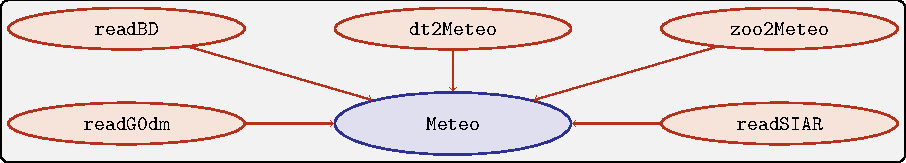
\includegraphics[keepaspectratio,width=\textwidth,height=0.5\textheight]{figuras/meteo.pdf}
\caption{Los datos meteorologicas se pueden leer mediante las funciones \texttt{readG0dm}, \texttt{readBD}, \texttt{dt2Meteo}, \texttt{zoo2Meteo} y \texttt{readSIAR} las cuales procesan estos datos y los almacenan en un objeto de clase \texttt{Meteo}. \label{fig:meteo}}
\end{figure}
\begin{itemize}
\item \texttt{readG0dm}: Esta función construye un objeto \texttt{Meteo} a partir de 12 valores de medias mensuales de irradiación.
\end{itemize}
\begin{lstlisting}[numbers=left,language=r,label= ,caption= ,captionpos=b]
G0dm =
  c(2.766,3.491,4.494,5.912,6.989,7.742,7.919,7.027,5.369,3.562,2.814,2.179) * 1000;
Ta = c(10, 14.1, 15.6, 17.2, 19.3, 21.2, 28.4, 29.9, 24.3, 18.2, 17.2, 15.2)
BD <- readG0dm(G0dm = G0dm, Ta = Ta, lat = 37.2)
print(BD)
\end{lstlisting}

\begin{verbatim}
Object of class  Meteo 

Source of meteorological information: prom- 
Latitude of source:  37.2 degrees

Meteorological Data:
     Dates                 G0d             Ta       
 Min.   :2024-01-17   Min.   :2179   Min.   :10.00  
 1st Qu.:2024-04-07   1st Qu.:3322   1st Qu.:15.50  
 Median :2024-06-29   Median :4932   Median :17.70  
 Mean   :2024-07-01   Mean   :5022   Mean   :19.22  
 3rd Qu.:2024-09-25   3rd Qu.:6998   3rd Qu.:21.98  
 Max.   :2024-12-13   Max.   :7919   Max.   :29.90
\end{verbatim}

\begin{itemize}
\item \texttt{readBD}: Esta familia de funciones puede leer ficheros de datos y transformarlos en un objeto de clase \texttt{Meteo}. Se dividen en:
\begin{itemize}
\item \texttt{readBDd}: Procesa datos meteorológicos de tipo diarios.
\end{itemize}
\begin{lstlisting}[numbers=left,language=r,label= ,caption= ,captionpos=b]
## Se utiliza un archivo alojado en github
myURL <-"https://raw.githubusercontent.com/oscarperpinan/R/master/data/aranjuez.csv"
## Se emplea un archivo temporal
temp_file <- tempfile(tmpdir = '') 
download.file(myURL, temp_file, quiet = TRUE)
BDd <- readBDd(file = temp_file, lat = lat, format = '"exports both"Y/"exports both"m/"exports both"d', header = TRUE,
               fill = TRUE, dec = '.', sep = ',', dates.col = '',
               ta.col = 'TempAvg', g0.col = 'Radiation', keep.cols = TRUE)
unlink(temp_file)
print(BDd)
\end{lstlisting}

\begin{verbatim}
Object of class  Meteo 

Source of meteorological information: bd-\filec94adc23fb 
Latitude of source:  40 degrees

Meteorological Data:
     Dates            G0               Ta            TempMin           TempMax          HumidAvg     
 Min.   :NA     Min.   : 0.277   Min.   :-5.309   Min.   :-12.980   Min.   :-2.362   Min.   : 19.89  
 1st Qu.:NA     1st Qu.: 9.370   1st Qu.: 7.692   1st Qu.:  1.515   1st Qu.:14.530   1st Qu.: 47.04  
 Median :NA     Median :16.660   Median :13.810   Median :  7.170   Median :21.670   Median : 62.58  
 Mean   :NaN    Mean   :16.742   Mean   :14.405   Mean   :  6.888   Mean   :22.531   Mean   : 62.16  
 3rd Qu.:NA     3rd Qu.:24.650   3rd Qu.:21.615   3rd Qu.: 12.590   3rd Qu.:30.875   3rd Qu.: 77.38  
 Max.   :NA     Max.   :32.740   Max.   :30.680   Max.   : 22.710   Max.   :41.910   Max.   :100.00  
 NA's   :2898   NA's   :13                        NA's   :4                                          
    HumidMax         WindAvg         WindMax            Rain              ET       
 Min.   : 35.88   Min.   :0.251   Min.   : 0.000   Min.   : 0.000   Min.   :0.000  
 1st Qu.: 81.60   1st Qu.:0.667   1st Qu.: 3.783   1st Qu.: 0.000   1st Qu.:1.168  
 Median : 90.90   Median :0.920   Median : 5.027   Median : 0.000   Median :2.758  
 Mean   : 87.22   Mean   :1.174   Mean   : 5.208   Mean   : 1.094   Mean   :3.091  
 3rd Qu.: 94.90   3rd Qu.:1.431   3rd Qu.: 6.537   3rd Qu.: 0.200   3rd Qu.:4.926  
 Max.   :100.00   Max.   :8.260   Max.   :10.000   Max.   :49.730   Max.   :8.564  
 NA's   :13       NA's   :8       NA's   :128      NA's   :4        NA's   :18
\end{verbatim}

\begin{itemize}
\item \texttt{readBDi}: Procesa datos meteorológicos de tipo intradiarios.
\end{itemize}
\item \texttt{dt2Meteo}: Transforma un \texttt{data.table} o \texttt{data.frame} en un objeto de clase \texttt{Meteo}.
\item \texttt{zoo2Meteo}: Transforma un objeto de clase \texttt{zoo}\footnote{Pese a que este proyecto trate de ``desligarse'' del paquete \texttt{zoo}, sigue siendo un paquete muy extendido. Por lo que es interesante tener una función así para que los usuarios tengan una mayor flexibilidad.} en un objeto de clase \texttt{Meteo}.
\item \texttt{readSIAR}: Esta función es capaz de extraer información de la red SIAR y transformarlo en un objeto de clase \texttt{Meteo}.
\end{itemize}

\subsection{Radiación en el plano horizontal.}
\label{sec:org129992b}
\begin{enumerate}
\item La información de irradiación en el plano horizontal (en todos sus componentes o, en su defecto, solo la global(\(G_d(0)\))) y temperatura viene dada en un objeto de clase \texttt{Meteo}.
\item Mediante la función fCompD, se calcula:
\begin{itemize}
\item La fracción de radiación difusa diaria (\(F_{Dd}\)).
\item El índice de claridad diario (\(K_{Td}\)).
\item Si solo se tienen datos de la componente global de irradición:
\begin{itemize}
\item La irradiación directa en el plano horizontal (\(B_d(0)\)).
\item La irradiación difusa en el plano horizontal (\(D_d(0)\)).
\end{itemize}
\end{itemize}
\item Mediante la función fCompI, se calcula:
\begin{itemize}
\item La fracción de radiación difusa (\(F_D\)).
\item El índice de claridad (\(K_T\)).
\item Si solo se tienen datos de la componenete global de irradiancia (\(G(0)\)):
\begin{itemize}
\item La irradiancia directa en el plano horizontal (\(B(0)\)).
\item La irradiancia difusa en el plano horizontal (\(D(0)\)).
\end{itemize}
\end{itemize}
\item El resultado de ambas funciones junto a medias mensuales y valores anuales se consolidan en un solo objeto de clase \texttt{G0} (que incluye los objetos \texttt{Sol} y \texttt{Meteo} de los que parte) mediante la función calcG0.
\end{enumerate}
\subsection{Radiación en el plano del generador.}
\label{sec:orgfc8b90d}
\begin{enumerate}
\item La información de radiación puede venir dada en forma de un objeto de clase \texttt{Meteo} o un objeto de clase \texttt{G0} (ya que es este último el que se necesita para estimar la radiación en el plano del generador).
\item Mediante la función fTheta, se calcula:
\begin{itemize}
\item Ángulo de inclinación de la superficie del módulo (\(\beta\)).
\item Ángulo azimutal de la superficie del módulo (\(\alpha\) ).
\item Ángulo de incidencia de la irradiancia solar en la superficie del módulo (\(\theta_s\)).
\end{itemize}
\item Mediante la función fInclin, se calcula:
\begin{itemize}
\item La irradiancia extra-terrestre en la superficie inclinada (\(B_0(\beta, \alpha)\)).
\item La irradiancia directa normal (\(B(n)\)).
\item Las irradiancias global (\(G(\beta, \alpha)\)), directa (\(B(\beta, \alpha)\)), difusa (\(D(\beta, \alpha)\))(total, isotropica y anisotrópica) y del albedo (\(R(\beta, \alpha)\)) sobre una superficie inclinada.
\item Las irradiancias efectivas global (\(G_{ef}(\beta, \alpha)\)), directa (\(B_{ef}(\beta, \alpha)\)), difusa (\(D_{ef}(\beta, \alpha)\))(total, isotropica y anisotrópica) y del albedo (\(R_{ef}(\beta, \alpha)\)) sobre una superficie inclinada.
\item Los factores de pérdidas angulares para las componentes directa (\(FT\)), difusa (\(FT_D\)), y del albedo (\(FT_R\)).
\end{itemize}
\item Mediante la función calcShd, se puede calcular:
\begin{itemize}
\item La irradiancia e irradiación incluyendo sombras para seguidores a dos ejes y horizontales y paneles fijos mediante la función fSombra.
\end{itemize}
\item El resultado de estas funciones junto a medias mensuales y valores anuales se consolidan en un solo objeto de clase \texttt{Gef} (que incluye el objeto \texttt{G0} del que parte) mediante la función calcGef.
\end{enumerate}
\subsection{Producción eléctrica.}
\label{sec:orgb4afcdb}
\begin{enumerate}
\item Mediante la función fProd, se calcula:
\begin{itemize}
\item La potencia en corriente continua (\(P_{DC}\)).
\item La potencia en corriente alterna (\(P_{AC}\)).
\end{itemize}
\item Estos resultados, llevados a valores diarios, mensuales y anuales, se pueden convertir en valores de energía (\(E_{DC}\) y \(E_{AC}\)) y de productividad del sistema (\(Y_f\)), los cuales se consolidan en un solo objeto de clase \texttt{ProdGCPV} (que incluye el objeto \texttt{Gef} del que parte) mediante la función prodGCPV.
\end{enumerate}
